\providecommand{\InstrumentMoneyMark}{%
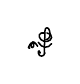
\begin{tikzpicture}[x=.024em,y=-.024em,baseline=-.72em,line width=.055em,line cap=round,line join=round]
\path[use as bounding box] (0,0) rectangle (37,43);
\draw (25,39) .. controls (25,28) and (26,12) .. (26,5)
 .. controls (26,-2) and (32,-1) .. (33,5)
 .. controls (35,12) and (33,17) .. (28,18);
\draw (26,8) .. controls (17,6) and (15,13) .. (20,18)
 .. controls (25,23) and (35,21) .. (36,15)
 .. controls (37,11) and (33,8) .. (29,8);
\draw (16,22) .. controls (21,31) and (31,32) .. (36,24);
\draw (26,38) .. controls (25,44) and (17,45) .. (16,38)
 .. controls (15,34) and (19,34) .. (19,38);
\draw (15,28) .. controls (12,23) and (8,19) .. (6,23)
 .. controls (3,28) and (7,33) .. (9,28)
 .. controls (10,22) and (5,21) .. (3,26)
 .. controls (0,29) and (1,32) .. (3,31);
\end{tikzpicture}}
